\section{Linear Regression}

Implementing linear regression was the first part of the assignment.

\subsection{Introduction}



\subsection{Questions}

\subsubsection{Question 1: What weight vector was calculated using gradient descent?}

We got the weight vector $w = [0.4154, 5.2012, 2.0025]$ for the sample problem after 1000 iterations of gradient descent with the learning rate $\gamma = 0.001$.

\subsubsection{Question 2: How can you calculate the optimal weight directly? How much different is it to the result of gradient descent?}

We can use linear algebra to reformulate the gradient descent problem. After solving the formula we get $w = (XX^T)^{-1}Xt^T$. Therefore, if $XX^T$ is invertible we can use this formula to directly compute the optimal weight vector.

Our test data is randomly generated and the variance to the real data is also at random, therefore the weight vector had small differences in distances to each other. With this procedure we got t the optimal weight vector $w^* = [0.4040, 5.2352, 1.9910]$, whereby the gradient descent weight vector was $w = [0.4154, 5.2012, 2.0025]$. This result was obtained with the same testdata, we had used for question 1. 

\begin{figure}[!ht]
	\centering
	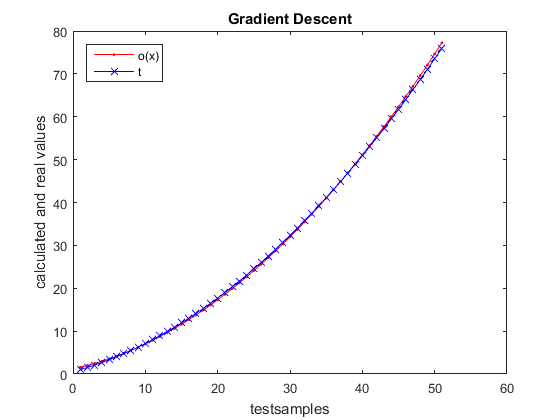
\includegraphics[width=0.5\textwidth]{img/gradientDescent}
	\caption{Performance by gradient descent on the real dataset}
	\label{perGraDescent}
\end{figure}


\begin{figure}[!ht]
	\centering
	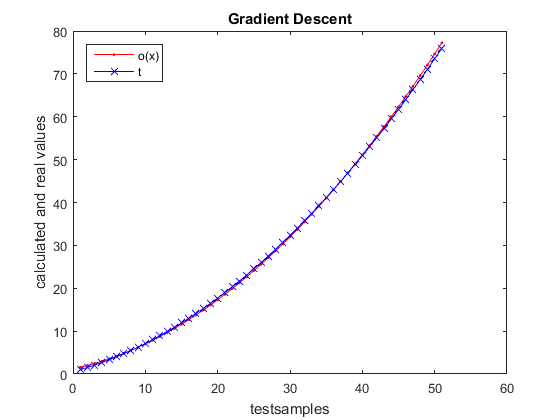
\includegraphics[width=0.5\textwidth]{img/gradientDescent}
	\caption{Performance by gradient descent on the real dataset}
	\label{perGraDescent}
\end{figure}



\subsubsection{Question 3: }





